\documentclass[presentation.tex]{subfiles}


\begin{document}
	\begin{frame}[fragile]
		\frametitle{Nadstavba}
                \begin{python}
from models.models import L1Model, LInfModel
                \end{python}
        \begin{columns}
            \begin{column}{0.5\textwidth}
                \begin{itemize}
                    \item Zovšeobecnenie problému
                    \item Voľnosť dimenzionality
                    \item Vstupný vektor $y$ a matica $X$
                    \item Hodnoty $\beta$ výstupom
                \end{itemize}
            \end{column}

            \begin{column}{0.5\textwidth}
                \begin{python}
# inicializacia
model1 = L1Model(y, X)
model2 = LInfModel(y, X)
# riesenie
beta1 = model1.solve()
beta2 = model2.solve()
                \end{python}
            \end{column}
        \end{columns}
	\end{frame}

    \begin{frame}[fragile]
        \frametitle{Nadstavba}
        \begin{multicols}{2}
            \begin{itemize}
                    \item Hodnota $R^2$
                    \item \pyth|model.r2()|
            \end{itemize}

            \columnbreak

            \begin{itemize}
                    \item Vizualizácia pre 2D a 3D
                    \item \pyth|model.visualize()|
            \end{itemize}
        \end{multicols}

        \begin{columns}
            \begin{column}{0.5\textwidth}
                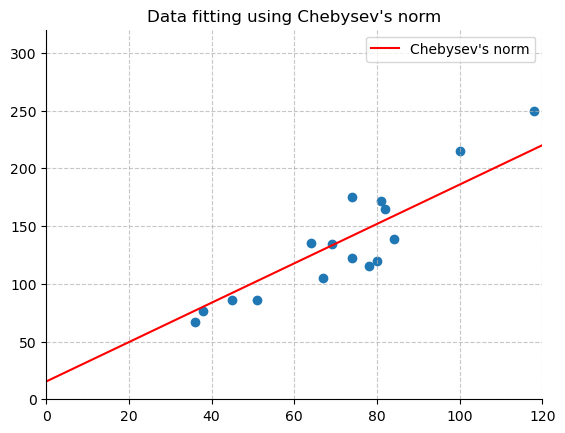
\includegraphics[width=1\linewidth]{2D_viz.png}
            \end{column}
            \begin{column}{0.5\textwidth}
                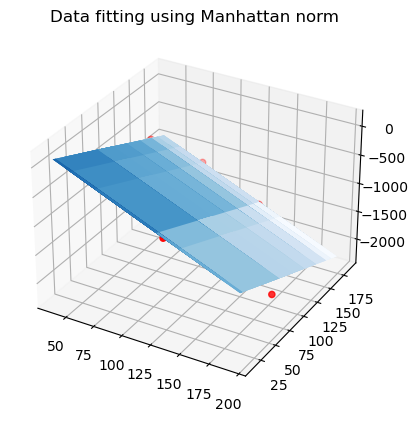
\includegraphics[height=140, width=0.9\linewidth]{3D_viz.png}
            \end{column}
        \end{columns}
    \end{frame}
\end{document}